\documentclass{article}
% NeurIPS 2025 style (neurips_2025.sty, in this folder) as a preprint: author names shown, no line numbers.
\usepackage[preprint,nonatbib]{neurips_2025}
\usepackage[utf8]{inputenc}
\usepackage[T1]{fontenc}
\usepackage{amsmath,amssymb}
\usepackage{booktabs}
\usepackage{array}
\usepackage{graphicx}
\usepackage[numbers,sort&compress]{natbib}
\usepackage{hyperref}
\hypersetup{colorlinks=true,linkcolor=blue!50!black,citecolor=blue!50!black,urlcolor=blue!50!black}
\usepackage{xcolor}
\usepackage{microtype}
% Generated by paper2/make_assets.py from results/multiagent/; do not edit by hand.
\newcommand{\BoardBenefitEight}{0.60}
\newcommand{\BoardBenefitEightCI}{[0.57, 0.63]}
\newcommand{\ColonyNoCall}{2}
\newcommand{\ColonyPredBoard}{+0.29}
\newcommand{\ColonyPredGuards}{-0.040}
\newcommand{\ColonyRight}{3}
\newcommand{\ColonyWrong}{1}
\newcommand{\CostPhaseEleven}{3.56}
\newcommand{\CostPhaseTen}{32.68}
\newcommand{\ForageBenefitEight}{-0.34}
\newcommand{\ForageBenefitEightCI}{[-0.48, -0.13]}
\newcommand{\ForecastAgree}{4}
\newcommand{\ForecastTotal}{8}
\newcommand{\LiarCredit}{0.500}
\newcommand{\LiarCreditCI}{[0.280, 0.625]}
\newcommand{\LiarWarm}{0.311}
\newcommand{\LiarWarmCI}{[0.189, 0.399]}
\newcommand{\NumpySeeds}{30}
\newcommand{\NumpyWallMinutes}{5}
\newcommand{\ObsCredturnWelfare}{+0.069}
\newcommand{\ObsCredturnWelfareCI}{[+0.018, +0.120]}
\newcommand{\ObsIndpenShare}{+0.002}
\newcommand{\ObsIndpenShareCI}{[-0.038, +0.042]}
\newcommand{\ObsIndpenWelfare}{+0.053}
\newcommand{\ObsIndpenWelfareCI}{[+0.000, +0.106]}
\newcommand{\PredCredturnWelfare}{+0.037}
\newcommand{\PredIndShare}{-0.486}
\newcommand{\PredIndpenShare}{-0.477}
\newcommand{\PredIndpenWelfare}{-0.062}
\newcommand{\RetroAgree}{7}
\newcommand{\RetroTotal}{12}
\newcommand{\RhoBoard}{0.75}
\newcommand{\RhoBoardCI}{[0.55, 0.93]}
\newcommand{\RhoClue}{0.79}
\newcommand{\RhoClueCI}{[0.74, 0.81]}
\newcommand{\RhoForage}{0.02}
\newcommand{\RhoForageCI}{[-0.47, 0.45]}
\newcommand{\ScaleAgree}{1}
\newcommand{\ScaleObsLoss}{+0.076}
\newcommand{\ScaleObsLossCI}{[+0.013, +0.137]}
\newcommand{\ScaleObsPool}{-0.065}
\newcommand{\ScaleObsPoolCI}{[-0.081, -0.048]}
\newcommand{\ScalePredLoss}{-0.134}
\newcommand{\ScalePredPool}{-0.156}
\newcommand{\ScaleTotal}{2}
\newcommand{\TestHOne}{-7.545}
\newcommand{\TestHOneCI}{[-8.101, -7.030]}
\newcommand{\TestHOneP}{0.0003}
\newcommand{\TestHThree}{0.041}
\newcommand{\TestHThreeCI}{[0.033, 0.049]}
\newcommand{\TestHThreeP}{0.0001}
\newcommand{\TestHTwo}{-0.109}
\newcommand{\TestHTwoCI}{[-0.111, -0.108]}
\newcommand{\TestHTwoP}{0.0003}
\newcommand{\TestP}{0.091}
\newcommand{\TestPCI}{[0.088, 0.093]}
\newcommand{\TestPP}{0.0003}
\newcommand{\TraceContamEight}{0.79}
\newcommand{\TraceContamThirtyTwo}{0.91}
\newcommand{\TraceHaikuChange}{+0.08}
\newcommand{\TraceHaikuPoisonEight}{0.25}
\newcommand{\TraceHaikuPoisonThirtyTwo}{0.31}
\newcommand{\TraceHaikuPoolEight}{0.41}
\newcommand{\TraceHaikuPoolThirtyTwo}{0.34}
\newcommand{\TraceHaikuUntouchedEight}{0.26}
\newcommand{\TraceHaikuUntouchedThirtyTwo}{0.27}
\newcommand{\TraceNumpyPoisonEight}{0.37}
\newcommand{\TraceNumpyPoisonThirtyTwo}{0.37}
\newcommand{\TraceNumpyPoolEight}{0.51}
\newcommand{\TraceNumpyPoolThirtyTwo}{0.36}
\newcommand{\TraceNumpyUntouchedEight}{0.37}
\newcommand{\TraceNumpyUntouchedThirtyTwo}{0.23}
\newcommand{\TracePlanHash}{f5c25637acd0}
\newcommand{\TraceRelayMax}{0.25}
\newcommand{\TraceShareAC}{0.72}
\newcommand{\TraceShareACCI}{[0.16, 3.2]}
\newcommand{\TraceSuppress}{89--94}
\newcommand{\TraceVarFirst}{-0.16}
\newcommand{\TraceVarRelay}{-0.23}
\newcommand{\TraceVarRepost}{-0.05}
\newcommand{\TraceWrongContam}{95--97}


\title{Simulate First? What Cheap Rule-Agent Worlds Predict About Teams of Language-Model Agents}

\author{%
  Chuntao Dan \\
  \And
  Claude Opus 5.5\thanks{An AI model made by Anthropic, working as a research and coding agent in Claude Code; see the author contributions.} \\
  Anthropic \\
}

\begin{document}
\maketitle

\begin{abstract}
Every design choice for a team of language-model agents (how agents communicate, how many there are, who checks whom, how they are rewarded) is expensive to test with real models. We ask whether a cheap, hand-built simulation, not fitted to any language model, can screen these choices first, and score its forecasts, frozen before the expensive runs, against five findings of a companion paper about teams of up to 64 Claude Haiku 5.5 agents and reinforcement learning (RL) of a 3B open-weight model. Where a finding is about how information flows or how a team is structured, the simulation was a good screen: rule-agent worlds ranked harness designs as Haiku teams did on a task board ($\rho = \RhoBoard$) and a clue board ($\rho = \RhoClue$), though not on foraging described in text ($\rho = \RhoForage$), and its forecasts for three studies of defences against liars were right on $\ColonyRight$ of $\ColonyCalled$, $\FourRight$ of $\FourCalled$ and $\FourBRight$ of $\FourBCalled$ effects with a clear outcome, including that splitting a large team into squads would keep a defence from fading as teams grow. Where a finding depends on what language models do, it missed: it predicted that agents assigned as guards would cost more than they protect (they were the strongest defence), that larger teams would lose less to liars (they lost more), and that dealing guards one copy of every clue would hurt at 64 agents (it helped). For reward designs, its effects had the same sign as the LLM's in $\RetroAgree$ of $\RetroTotal$ cases for runs already completed and $\ForecastAgree$ of $\ForecastTotal$ for runs not yet made. Simulations are a useful screen for information flow and team structure, and a poor one for what language models learn in training, how they read shared text, or what they do in a role.
\end{abstract}

\section{Introduction}

Agent teams are designed by trial and error over channels (a shared board, peer messages, a coordinator), team size and structure, roles, memory and incentives. With real models each trial costs API calls or GPU hours; with RL, a single run can take hours and, as our companion paper shows, results can vary as much between training seeds as between designs. Cheap simulations are the obvious screen, but whether they transfer to language-model agents is an empirical question. Surrogates fitted to an LLM's own decisions can reproduce the macro outcomes of LLM societies \citep{itkin2026poorman}, and machine-learning surrogates can stand in for classic agent-based models \citep{angione2022surrogate}; across 260 configurations of real agent systems, a feature-based model picks the best architecture in most held-out cases \citep{kim2025scaling}. We test a different and cheaper route: hand-built worlds with simple agents that are \emph{not} fitted to any LLM, used to rank designs and to forecast effects before the expensive runs.

The companion paper reports five findings about large teams of language-model agents: (1) verification works as an assigned role; (2) splitting a large team into squads makes verification scale; (3) larger teams are more gullible; (4) copies of one model do not divide labour on their own, and the reward decides whether trained copies cooperate; (5) mechanisms that move information without costing turns help, while those that add work to every agent's turn do not. Our contributions: (i) for each finding, what a cheap simulation predicted before the runs, scored with a frozen rule (Table~\ref{tab:findings}); (ii) design rankings that transfer from rule-agent worlds to Claude Haiku 5.5 teams on two of three tasks, with one clear failure; (iii) pre-registered confirmatory tests of four hypotheses about shared information in the simulation, all supported; (iv) a practical workflow for when to trust the screen.

\section{Methods}
\label{sec:methods}

\paragraph{The foraging world.} Agents move between resource patches on a ring or torus, share each patch's intake when they crowd it, and pay travel time; patches move, so agents must keep exploring. Each agent is a UCB bandit over locations. Channels: none; a \emph{blackboard} (a shared map of each location's value); \emph{messages} (each agent sends a few location-value reports to peers); a \emph{coordinator} that collects reports and assigns agents. Team sizes run from 1 to 64 under two budgets: fixed compute (total agent-seconds held constant) and fixed world time. The ideal free distribution \citep{fretwell1969ifd}, in which no agent can gain by moving, is the reference for how well agents spread over patches. A scripted liar posts false patch values. Hypotheses and the analysis were frozen and hashed before the runs; each test used $\NumpySeeds$ seeds and Holm correction.

\paragraph{The task board, text foraging and the clue board.} The same channels were given to Claude Haiku 5.5 teams of 1 to 8 agents on a task board, where the risk is duplicate work, and on foraging described in text. On the clue board, information is the bottleneck: each subtask's answer is fixed by two modular clues dealt to different agents, so nobody can solve it alone and sharing costs a turn; the \emph{pooled share} is a team's welfare as a share of what it would earn if every clue were known to all. Numpy rule agents played the same tasks for the comparison.

\paragraph{Defences against liars.} On the clue board with each clue held by two agents and a quarter of the agents liars, numpy rule agents played the companion paper's defences against the \emph{plain board} (no defence): a board that counts how many agents posted each value (the \emph{counting board}), guards (agents who post, confirm and contest clues and never solve), and three changes meant to make guards scale (squads of eight, each with its own board, subtasks and guards; flags on posted values that a wrong answer agreed with; and \emph{guard copies}, which deal one of each clue's two copies to a guard), at 8 to 128 agents with 30 seeds.

\paragraph{Reward designs.} A 3B open-weight model (Qwen2.5-3B-Instruct), warm-started by imitating a rule agent, was trained with group-relative policy gradient on the clue board under five reward designs: individual (an agent's own points), team (the team's mean), credit (the solver shares a subtask's value with the agents whose clues it used), individual with a training-only penalty on wrong answers (\texttt{indpen}: a wrong answer costs 3 instead of 0.5), and credit with per-turn advantages and the same penalty (\texttt{credturn}). The numpy counterpart is the rule agent with two learned choices, whether to share a clue it could share and whether to guess on an undetermined subtask, trained by the same policy gradient under the same five rewards from a start that imitates the rule agent imperfectly, as the LLM's warm start does. Both are measured by welfare, shares per held clue, the \emph{solo share} (solves made by guessing while several candidate answers remained) and wrong answers per solve.

\paragraph{Forecasts and scoring.} Every forecast and its scoring rule were committed before the runs it predicts. A forecast's sign is + or $-$ when its 95\% interval over seeds excludes zero, and 0 otherwise. Against the Haiku result, a forecast is \emph{right} when the Haiku interval excludes zero on the predicted side, \emph{wrong} when the Haiku interval excludes zero but the forecast had the other sign or 0, and \emph{inconclusive} when the Haiku interval spans zero; scores count right forecasts among the conclusive ones. Reward forecasts are scored instead by whether the simulation's sign matches the LLM's, 0 matching 0.

\paragraph{Statistics.} Rank agreement is Spearman's $\rho$ between the simulation's and the LLM teams' means over the (channel, team size) cells of a task, with a 95\% bootstrap interval resampling seeds. The four confirmatory hypotheses in the simulation were tested with paired sign-flip tests and Holm correction under a plan frozen before the runs. In the text, brackets give 95\% bootstrap intervals over seeds. In the figures, points are means, error bars are one standard error of the mean (SEM) over seeds, and an asterisk marks $p < 0.05$ in a two-sided sign-flip test against the stated reference (exact when the sign patterns number at most $2^{15}$, otherwise 40{,}000 random flips), uncorrected.

\section{Results}

\begin{table}[t]
\centering
\small
\begin{tabular}{@{}>{\raggedright\arraybackslash}p{2.9cm}>{\raggedright\arraybackslash}p{7.6cm}>{\raggedright\arraybackslash}p{2.3cm}@{}}
\toprule
Finding (companion paper) & What the frozen simulation said & Score \\
\midrule
1. Verification as an assigned role & the counting board helps, cuts answers built on lies and costs output on boards without liars (right); guards cost more than they protect (wrong) & $\ColonyRight$ of $\ColonyCalled$ \\
2. Squads make verification scale & squads beat guards on one board and lose less ground than them as teams grow; flags help; guard copies lose less ground with size (right); guard copies hurt at 64 agents (wrong) & $\FourRight$ of $\FourCalled$; at 32 agents $\FourBRight$ of $\FourBCalled$ \\
3. Larger teams are more gullible & pooling falls with size (right); loss to liars falls with size (wrong) & $\ScaleAgree$ of $\ScaleTotal$ \\
4. Rewards decide cooperation & individual reward drifts selfish (right); a wrong-answer penalty fails to stop it (scored wrong, later seed-dependent) & retrodiction $\RetroAgree$ of $\RetroTotal$; forecast $\ForecastAgree$ of $\ForecastTotal$ \\
5. Move information, do not add work & rank agreement on two of three tasks ($\rho = \RhoBoard$, $\RhoClue$; foraging $\RhoForage$) & --- \\
\bottomrule
\end{tabular}
\caption{What a cheap rule-agent simulation predicted about each finding, forecasts frozen before the runs. Scores count right forecasts among effects with a conclusive Haiku result (\S\ref{sec:methods}); the reward row gives the retrodiction (runs already completed) and the forecast (runs not yet made) separately.}
\label{tab:findings}
\end{table}

\subsection{Information flow: rankings and confirmatory tests (finding 5)}

\begin{table}[h]
\centering
\small
\begin{tabular}{@{}>{\raggedright\arraybackslash}p{6.1cm}ccc@{}}
\toprule
Test (blackboard minus no channel; H3: blackboard minus messages) & Mean [95\% CI] & Holm $p$ & Verdict \\
\midrule
P (primary): welfare per agent-second, $N$ 2--64, fixed compute & $\TestP$ $\TestPCI$ & $\TestPP$ & supported \\
H1: recovery time to the ideal free distribution (s) & $\TestHOne$ $\TestHOneCI$ & $\TestHOneP$ & supported \\
H2: belief diversity (spread of agents' value estimates) & $\TestHTwo$ $\TestHTwoCI$ & $\TestHTwoP$ & supported \\
H3: honest agents' loss from one liar & $\TestHThree$ $\TestHThreeCI$ & $\TestHThreeP$ & supported \\
\bottomrule
\end{tabular}
\caption{Pre-registered tests in the numpy foraging world ($\NumpySeeds$ seeds each, run once against the frozen plan).}
\label{tab:tests}
\end{table}

In the simulation the blackboard keeps output per agent up as the team grows, speeds recovery after patches move, makes agents think alike, and makes the team more vulnerable to a liar than peer messages do (Table~\ref{tab:tests}, Figure~\ref{fig:sim}); the main grid ran in about $\NumpyWallMinutes$ minutes on a laptop. On the task board a shared claim board kept welfare per agent-turn flat as Haiku teams grew, adding $\BoardBenefitEight$ $\BoardBenefitEightCI$ over no channel at eight agents, and the simulation ranked the 16 (channel, team size) cells as the LLM teams did ($\rho = \RhoBoard$ $\RhoBoardCI$). On the clue board the agreement was as strong ($\rho = \RhoClue$ $\RhoClueCI$ over 12 cells); its main misses were the coordinator cells, where rule agents follow the coordinator and Haiku agents mostly ignored it. On text foraging the simulation failed ($\rho = \RhoForage$ $\RhoForageCI$): the blackboard \emph{hurt} Haiku teams ($\ForageBenefitEight$ $\ForageBenefitEightCI$ at eight agents), with less exploration and lower belief diversity: the herding \citep{bikhchandani1992cascades} that H2's loss of diversity can cause, in a stronger form than in the simulation. H3's direction carried over to the 3B model: after its warm start it lost more to a liar on the blackboard than with messages (by $\LiarWarm$ $\LiarWarmCI$). The Haiku runs cost \$$\CostPhaseTen$ (task board and text foraging) and \$$\CostPhaseEleven$ (clue board); the simulations cost minutes of laptop time.

\begin{figure}[t]
\centering
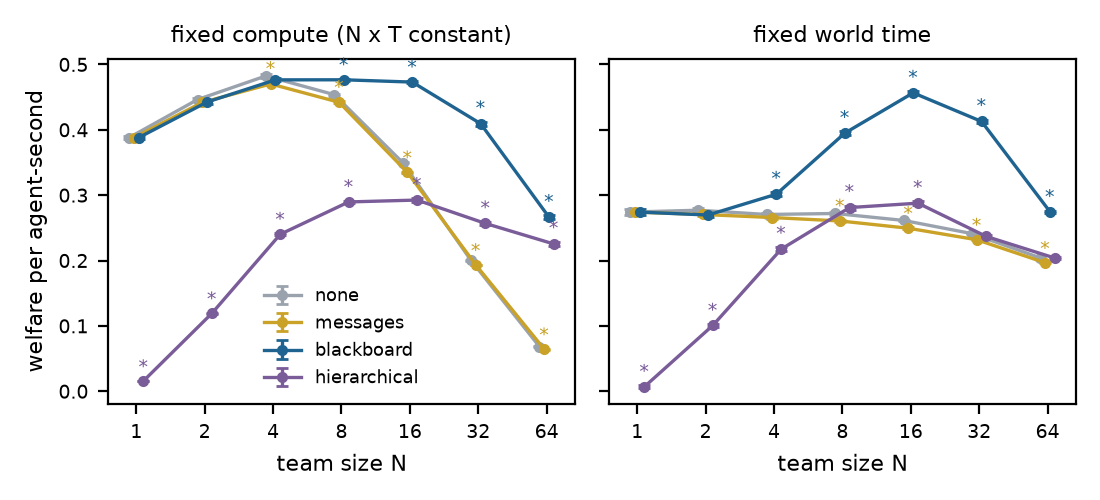
\includegraphics[width=\linewidth]{figures/scaling.png}\\[2pt]
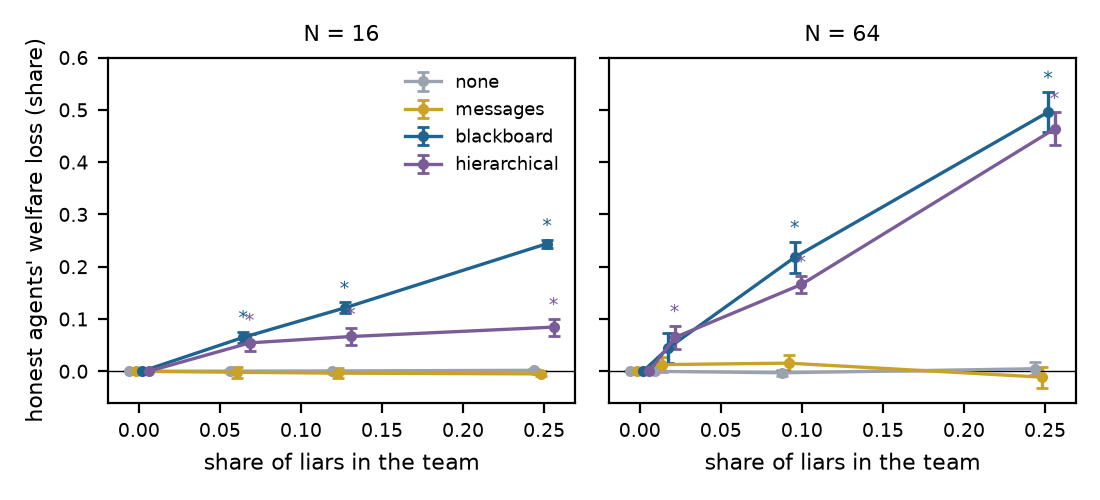
\includegraphics[width=\linewidth]{figures/robustness.png}
\caption{The numpy foraging world. Top: welfare per agent-second against team size under each channel, at fixed compute (total agent-seconds constant) and at fixed world time (30 seeds); * $p < 0.05$ against no channel at the same size, paired on seed. Bottom: the honest agents' welfare loss, as a share of their welfare without liars, against the share of liars at 16 and 64 agents (10 seeds); * $p < 0.05$ against no loss. Mean $\pm$ SEM; two-sided sign-flip tests (40{,}000 random flips over 30 seeds, exact over 10), uncorrected.}
\label{fig:sim}
\end{figure}

\subsection{Defences against liars (findings 1 and 2)}

Before Claude Haiku teams tried the defences, we froze a numpy forecast of $\ColonyPredTotal$ effects; of the $\ColonyScored$ that could be tested at 8 and 16 agents, it got $\ColonyRight$ right and $\ColonyWrong$ wrong, and $\ColonyNoCall$ were inconclusive. It was right that the counting board would help against liars (numpy $\ColonyPredBoard$), cut answers built on lies, and cost some output on boards without liars. It was wrong about the strongest effect: it predicted that guards would cost more than they protect (numpy $\ColonyPredGuards$), while Claude guards gained the most of any arm. Rule-agent guards only post what they hold and wait otherwise. With Claude guards, honest agents spent twice the share of their turns sharing ($\ColonyGuardsShareTurns$ against $\ColonyBoardShareTurns$ on the counting board alone), contested more lies ($\ColonyGuardsContests$ contests per lie against $\ColonyBoardContests$) and confirmed fewer of them ($\ColonyGuardsConfirms$ confirmations per lie against $\ColonyBoardConfirms$): behaviour the rule agents do not have.

Before the design changes meant to make guards scale, we froze a second forecast (30 seeds, 8 to 128 agents), scored on $\FourScored$ effects: $\FourRight$ right, $\FourWrong$ wrong and $\FourNoCall$ inconclusive. It got the structure right: squads would beat guards on one board at 64 agents (numpy $\FourPredSquads$; Haiku $\FourObsSquads$) and lose less ground than them from 16 to 64 agents (numpy $\FourPredDidSquads$; Haiku $\FourObsDidSquads$), with the squads' advantage over the plain board rising from $\FourNumpySquadsSixteen$ to $\FourNumpySquadsSixtyFour$ (Haiku $\FourObsSquadsSixteen$ to $\FourObsSquadsSixtyFour$) while that of guards on one board fell (numpy $\FourNumpyGuardsSixteen$ to $\FourNumpyGuardsSixtyFour$; Haiku $\FourObsGuardsSixteen$ to $\FourObsGuardsSixtyFour$); and failure flags would help (numpy $\FourPredFlags$; Haiku $\FourObsFlags$). It was wrong about guard copies at 64 agents (numpy $\FourPredCopies$; Haiku $\FourObsCopies$): in the simulation, dealing guards one copy of every clue leaves the other agents fewer clues, and guard copies trailed guards on one board at every size from 8 to 128 agents, while Claude guards turned the full coverage into a win at 64. For every effect it got right, its effect size was smaller than Haiku's, so it ranked the changes correctly but would have undersold the best one. A third forecast, for the same designs at 32 agents and drawn from the same frozen simulation before those runs, scored $\FourBRight$ right, $\FourBWrong$ wrong and $\FourBNoCall$ inconclusive: squads and failure flags beat guards on one board, as predicted, while guard copies, predicted to trail, drew level with them.

\subsection{Team-size trends (finding 3)}

Before running Claude Haiku teams of 8, 16 and 32 agents on the clue board, we froze a numpy forecast of how two measures would change from 8 to 32 agents. The simulation predicted that the pooled share of a team without liars would fall (numpy $\ScalePredPool$; Haiku $\ScaleObsPool$ $\ScaleObsPoolCI$) and that the honest agents' loss from a quarter of liars would fall too (numpy $\ScalePredLoss$), but it rose (Haiku $\ScaleObsLoss$ $\ScaleObsLossCI$): $\ScaleAgree$ of $\ScaleTotal$ right. Tracing every turn of both kinds of team (Haiku replayed from the response cache under a plan frozen first, with no API calls) and splitting the honest loss into exactly additive terms ruled out our first guess, that rule agents dilute a liar's posts among more true ones: lies were as visible at every size for both. The miss came from the trend without liars. Rule teams pool so much worse as they grow (pooled share $\TraceNumpyPoolEight$ to $\TraceNumpyPoolThirtyTwo$, against Haiku's $\TraceHaikuPoolEight$ to $\TraceHaikuPoolThirtyTwo$) that liars have less to take: the rule teams' loss on subtasks no lie touched fell from $\TraceNumpyUntouchedEight$ to $\TraceNumpyUntouchedThirtyTwo$ per agent-turn, while their loss on subtasks a lie touched stayed at $\TraceNumpyPoisonThirtyTwo$. Haiku's loss on untouched subtasks held ($\TraceHaikuUntouchedEight$ to $\TraceHaikuUntouchedThirtyTwo$) and its loss on touched ones grew ($\TraceHaikuPoisonEight$ to $\TraceHaikuPoisonThirtyTwo$), as its agents built on a false clue more often ($\TraceContamEight$ to $\TraceContamThirtyTwo$ of honest answers). Three rule-agent variants, each adding one candidate mechanism (passing on clues read from the board, trusting the first value posted, reposting a held clue until its true value is on the board), all still predicted a fall in the honest loss ($\TraceVarRelay$, $\TraceVarFirst$, $\TraceVarRepost$ against Haiku's $\TraceHaikuChange$; run after the fact): the error was in the baseline without liars, not in how rule agents handle lies.

\subsection{Reward designs (finding 4)}

Scored with the frozen rule (the sign of each arm's effect against the imitation start on the four measures), the numpy learners matched $\RetroAgree$ of $\RetroTotal$ signs in the runs already completed: $\RetroAgreeIndividual$ of 4 for individual reward (sharing changed by $\PredIndShare$ shares per held clue, guessing and wrong answers rose, welfare fell, as in the LLM run), $\RetroAgreeTeam$ of 4 for team reward (missing the LLM run's collapse) and $\RetroAgreeCredit$ of 4 for credit reward. The forecast for the two arms not yet run matched $\ForecastAgree$ of $\ForecastTotal$. It was right that RL with credit and per-turn advantages would raise welfare above the imitation start (numpy $\PredCredturnWelfare$; LLM $\ObsCredturnWelfare$ $\ObsCredturnWelfareCI$). It predicted that a training-only penalty on wrong answers would not stop the selfish drift under individual reward (sharing $\PredIndpenShare$), while the two scored LLM runs kept sharing ($\ObsIndpenShare$ $\ObsIndpenShareCI$); a later replication with $\SixteenPenRuns$ penalized runs found that effect seed-dependent ($\SixteenPenDrift$ of them drifted selfish), so this miss is less certain than its score. The simulation was not asked about the companion paper's last training result, that team reward did not make a division of labour emerge.

\section{Discussion}

\paragraph{When the simulation transfers.} It transferred where the mechanism is information flow or team structure that rule agents and language models handle alike: duplicate work avoided by a claim board, clues that must reach whoever needs them, a false report spread by a shared board, and smaller groups covering their own checking better than one large board. It failed where language models do something rule agents cannot: ignoring a coordinator's suggestion, herding in free text, keeping more of their performance without liars as teams grow (which leaves liars more to take), and contesting lies when given a guard's role. A recent taxonomy of when fitted surrogates work, by what agents perceive and remember \citep{itkin2026poorman}, offers a hypothesis to test: text gives LLM agents richer perception of others' behaviour than our rule agents have.

\paragraph{A practical workflow.} Use the simulation to rank channels, team sizes and team structures for tasks that turn on sharing information, and to flag incentive problems that come from who gets paid (it matched $\RetroAgreeIndividual$ of 4 signs of the selfish drift under individual reward); do not use it to rank reward designs that work through what the model learns about the team, to size the benefit of a role, or for tasks where reading shared text changes behaviour. Forecast an attack's effect separately from the trend without it, and check that trend first. When the simulation and a cheap LLM pilot disagree, the disagreement itself locates an LLM-specific behaviour worth studying: here, guards.

\paragraph{Future directions.} Three steps would make the screen more useful. (i) \emph{Hybrid simulations}: give the rule agents the behaviours the forecasts missed (treating a posted clue as settled, contesting lies in a role, ignoring a coordinator) as parameters fitted to a cheap LLM pilot, and test whether the hybrid forecasts the next study better than either the pure simulation or the pilot alone. (ii) \emph{More scored calls}: each study here added a handful of scored calls, too few to estimate calibration; forecasting every planned effect with a stated confidence would make calibration measurable. (iii) \emph{Free text and other model families}: our one ranking failure was the task with free text, where the gap between rule agents and language models should be largest, so the comparison should extend to text-heavy tasks and to other models before the screen is trusted there.

\paragraph{Limitations.} Three tasks with one LLM family for the rankings; one 3B model and two training seeds per reward design in the scored reward forecast; rank agreement over 12--16 cells; a simple numpy learner for the reward forecast. The frozen rule gave small, tight numpy effects a definite sign; with a post hoc practical-significance threshold (a numpy effect smaller than a tenth of the LLM warm start's value counts as 0), the reward scores are $\RetroAgreePostHoc$ of $\RetroTotal$ and $\ForecastAgreePostHoc$ of $\ForecastTotal$.

\section*{Author contributions}
Chuntao Dan directed the project: chose the questions and the order of the studies, made the design decisions recorded in the specifications, ran the GPU training and reviewed every result. Claude Opus 5.5, working as an agent in Claude Code under that direction, wrote the specifications, analysis plans, simulations, forecasts and analysis code, ran the API experiments and replays, analysed the results and drafted the paper. Chuntao Dan takes responsibility for the content.

\bibliographystyle{plainnat}
\bibliography{references}

\appendix
\section{Reproducibility}
Code and notebooks: \url{https://github.com/Positron00/explRL}. Confirmatory plans: Phase 8 \texttt{PREREG} (hash \texttt{8a59293847ae}) and Phase 9 \texttt{PREREG\_H3} (hash \texttt{a44617201f88}), frozen before their runs. The reward forecast: plan committed at \texttt{eb7b7c6}, predictions at \texttt{734839b}, both before the evaluated runs existed (\texttt{specs/multiagent/phase13/forecast.md}; \texttt{tools/rl\_forecast.py}, byte-identical on rerun). The team-size forecast: \texttt{tools/scale\_forecast.py}, committed before the Haiku runs. The colony-rule forecasts: \texttt{tools/colony\_forecast.py}; the first committed at \texttt{73557ea} before any Haiku run, the second (\texttt{colony4\_predictions.json}) at \texttt{1e9c53d} and the third, for 32 agents (\texttt{colony4b\_predictions.json}), at \texttt{6641a86}, each with its SHA-256 recorded in the frozen plan before its pilot. The traces that explain the team-size miss: \texttt{TRACE\_PLAN}, hash \texttt{\TracePlanHash}. Every number here is generated from the saved results by \texttt{paper2/make\_assets.py}, and every figure by \texttt{tools/figures.py}.

\end{document}
